\newpage
\section{Transport Layer}
\subsection{Overview of the transport layer}
Together with the network layer, the transport layer is the heart of the protocol hierarchy. The transport layer provides end-to-end connectivity across the network. 

\begin{figure}[!htb]
    \centering
    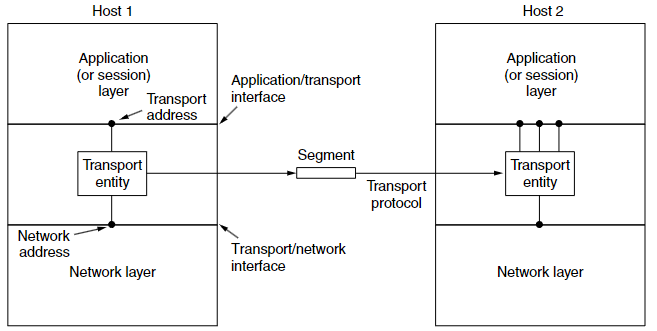
\includegraphics[width=0.42\textwidth]{pic/CN6/The network, transport, and application layers}
    \caption{The network, transport, and application layers}
\end{figure}

\subsubsection{The Transport Service}
Two types of transport service
\begin{itemize}
    \item Connection-oriented transport service
    \item Connectionless transport service
\end{itemize}
The transport code runs entirely on the users'machines, but the network layer mostly runs on the routers. The network service is generally unreliable. 

\subsubsection{Transit Units of Different Layers}
\begin{itemize}
    \item Transport layer: segment or TPDU (Transport Protocol Data Unit)
    \item Network layer: packet
    \item Data link layer: frame
    \item Physical layer: bit
\end{itemize}

\begin{figure}[!htb]
    \centering
    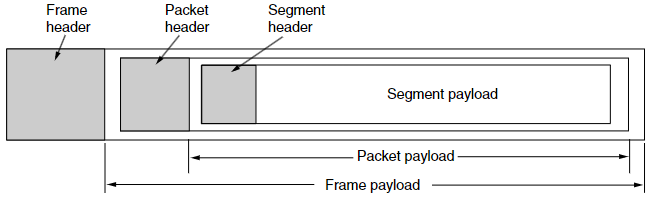
\includegraphics[width=0.42\textwidth]{pic/CN6/Nesting of segments, packets, and frames}
    \caption{Nesting of segments, packets, and frames}
\end{figure}

The Internet has two main protocols in the transport layer:
\begin{itemize}
    \item UDP (User Datagram Protocol, connectionless protocol): It does nothing beyond sending packets between applications. It typically runs in the operating system.
    \item TCP (connection-oriented protocol): It does almost everything. It makes connections and adds reliability with retransmission, along with flow control and congestion control.
\end{itemize}

\subsection{The internet transport protocols: UDP}
UDP: connectionless transport protocol. 

\begin{figure}[!htb]
    \centering
    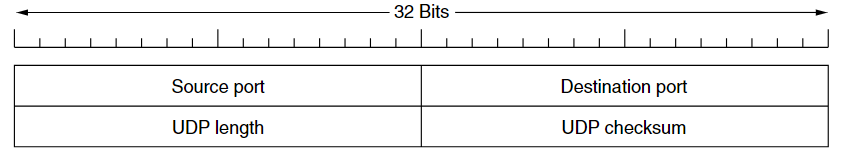
\includegraphics[width=0.42\textwidth]{pic/CN6/The UDP header}
    \caption{The UDP header}
\end{figure}

The two ports serve to identify the endpoints within the source and destination machines

\begin{itemize}
    \item UDP header (8 bytes)
    \begin{itemize}\small
        \item The UDP length field includes the 8-byte header and the data
        \subitem The minimum length is 8 bytes. The maximum length is 65,515 bytes. 
        \item The UDP checksum field (optional) is to provide extra reliability
        \subitem It checksums the header, data, and a conceptual IP pseudoheader
        \subitem The checksum algorithm is simply to add up all the 16-bit words (note here a word = 16 bits = 2 bytes) in one's complement and to take the one's complement of the sum.
    \end{itemize}
    \item The IPv4 pseudoheader
\end{itemize}
\begin{figure}[!htb]
    \centering
    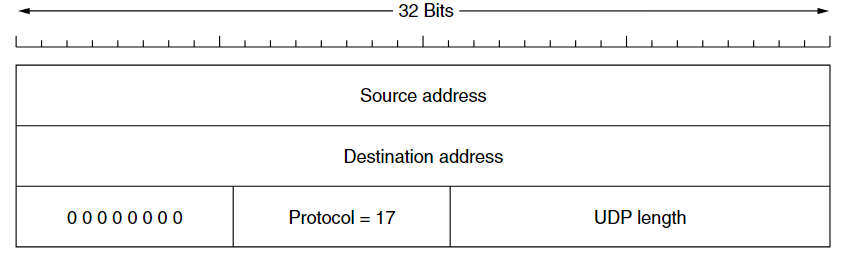
\includegraphics[width=0.42\textwidth]{pic/CN6/The IPv4 pseudoheader included in the UDP checksum.}
    \caption{The IPv4 pseudoheader included in the UDP checksum.}
\end{figure}

What UDP does not do: Flow control, congestion control, or retransmission upon receipt of a bad segment. 

What UDP does do:
\begin{itemize}
    \item To provide an interface to the IP protocol with the added feature of
    demultiplexing multiple processes using the ports.
    \item Optional end-to-end error detection (checksum)
\end{itemize}

The application uses the UDP protocol: 
\begin{itemize}
    \item DNS (Domain Name System, Chapter 7)
    \item SSDP (Simple Service Discovery Protocol)
\end{itemize}

\subsubsection{Real-Time Transport Protocol (RTP)}
It is a transport protocol but just happens to be implemented in the application layer.

Two aspects of real-time transport:
\begin{itemize}
    \item The RTP protocol for transporting audio and video data in packets
    \item How the receiver plays out the audio and video at the right time?
\end{itemize}

\begin{figure}[!htb]
    \centering
    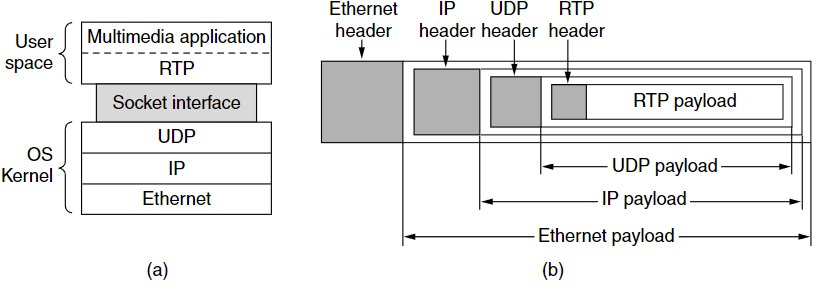
\includegraphics[width=0.42\textwidth]{pic/CN6/RTP.png}
    \caption{(a) The position of RTP in the protocol stack. (b) Packet nesting.}
\end{figure}

The basic function of RTP is to multiplex several real-time data streams onto a single stream of UDP packets

\begin{figure}[!htb]
    \centering
    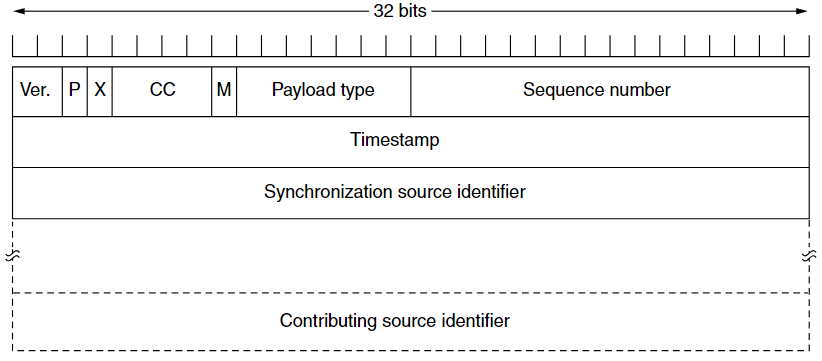
\includegraphics[width=0.42\textwidth]{pic/CN6/The RTP header}
    \caption{The RTP header}
\end{figure}
It consists of three 32- bit words and potentially some extensions
\begin{itemize}\small
    \item The Version field: 2
    \item The P bit indicates that the packet has been padded to a multiple of 4 bytes. The last padding byte tells how many bytes were added.
    \item The X bit indicates that an extension header is present.
    \item The CC field tells how many contributing sources are present, from 0 to 15.
    \item The M bit field is an application-specific marker bit.
    \item The Payload type field tells which encoding algorithm has been used.
    \item The Sequence number is just a counter that is incremented on each RTP packet sent. It is used to detect lost packets.
    \item The Timestamp is produced by the stream’s source to note when the 1st sample in the packet was made.
    \item The Synchronization source identifier tells which stream the packet belongs to.
    \item The Contributing source identifier, if any, are used when mixers are present in the studio.
\end{itemize}

\subsubsection{RTCP}
The RTCP (Real-time Transport Control Protocol) is a little sister protocol of RTP

Playout with Buffering and Jitter Control
\begin{figure}[!htb]
    \centering
    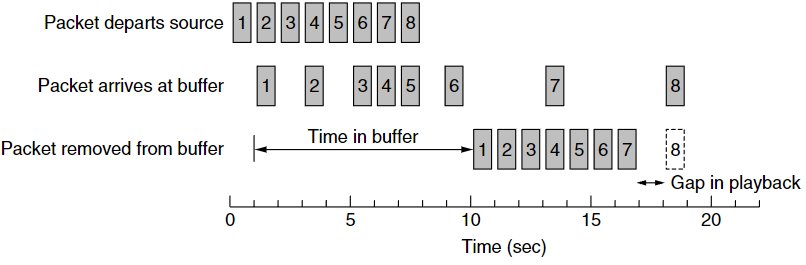
\includegraphics[width=0.42\textwidth]{pic/CN6/Smoothing the output stream by buffering packets}
    \caption{Smoothing the output stream by buffering packets}
\end{figure}

\subsection{The internet transport protocols: TCP}
TCP (Transmission Control Protocol) was designed to provide a reliable end-to-end byte stream over an unreliable internetwork. 

An internetwork may have wildly different topologies, bandwidths, delays, packet sizes, and other parameters in different parts.

\subsubsection{The TCP Service Model}
TCP service is obtained by both the sender and the receiver creating end points, called sockets. Each socket has a socket number (address) consisting of the IP addressing of the host and a 16-bit number local to that host, called a port.

All TCP connections are full duplex and point-to-point. TCP does not support multicasting and broadcasting. 

A TCP connection is a byte stream, not a message stream. (报文粘连问题)
\begin{figure}[!htb]
    \centering
    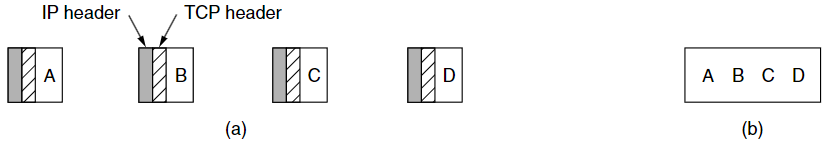
\includegraphics[width=0.42\textwidth]{pic/CN6/TCP connection is a byte stream}
    \caption{ (a) Four 512-byte segments sent as separate IP datagrams. (b) The 2048 bytes of data delivered to the application in a single READ call.}
\end{figure}

When an application passes data to TCP, TCP may send it immediately or buffer it.
\begin{itemize}
    \item PUSH flag: send immediately
    \item URGENT flag: high priority
\end{itemize}

\begin{figure}[!htb]
    \centering
    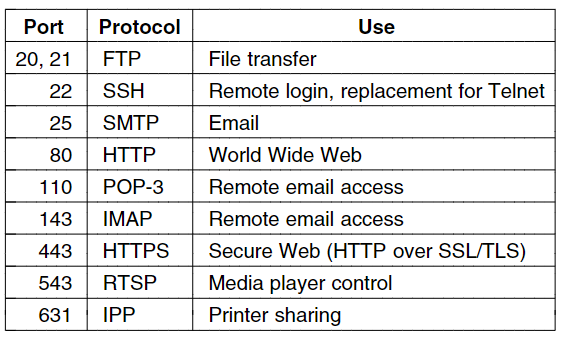
\includegraphics[width=0.309\textwidth]{pic/CN6/Some assigned ports}
    \caption{Some assigned ports}
\end{figure}

The TCP Protocol includes: a fixed 20-byte header + <optional> + <0-N data bytes>. 

The form of data exchange: segment. 

The basic TCP protocol: the sliding window protocol with dynamic window size. 

There are many problems to solve:
\begin{enumerate}
    \item Segment can arrive out of order
    \item Segments can also be delayed
\end{enumerate}

\subsubsection{The TCP Segment Header}
A key feature of TCP, and one that dominants the protocol design, is that every byte on a TCP connection has its own 32-bit sequence number. Every segment begins with a fixed-format, 20-byte header. 

Segments without any data are legal and are commonly used for acknowledgements and control messages.

\begin{figure}[!htb]
    \centering
    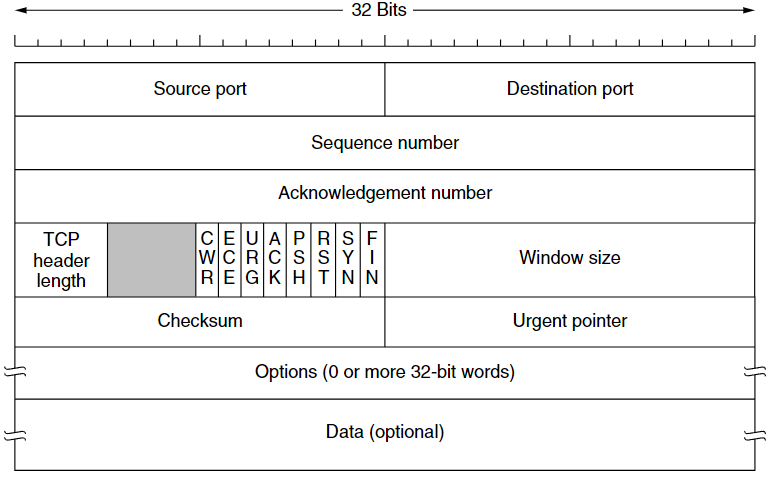
\includegraphics[width=0.42\textwidth]{pic/CN6/The TCP header}
    \caption{The TCP header}
\end{figure}

\begin{enumerate}
    \item The Source port (16 bits) and Destination port (16 bits)
    \subitem The connection identifier is a 5 tuple because it consists of five pieces of information: the protocol (TCP), source IP, and source port, and destination IP and destination port.
    \item The Sequence number (32 bits) and Acknowledgement number (32 bits) fields
    \subitem The Acknowledgement number specifies the next in-order byte expected, not the last byte correctly received.
    \subitem It is a cumulative acknowledgement because it summarizes the
    received data with a single number.
    \item The TCP header length (4 bits): because of the Options field. 
    \item The not used 4-bit field
    \item eight 1-bit fields (ack, syn, fin is important)
    \begin{itemize}\small
        \item CWR and ECE are used to signal congestion when ECN (Explicit Congestion Notification) is used.
        \subitem ECE is set to signal an ECN-Echo to a TCP sender
        \subitem CWR is set to signal Congestion Window Reduced from the TCP sender
        \item URG is set to 1 if the Urgent pointer is in use.
        \subitem The Urgent pointer is used to indicate which urgent data are to be found
        \item The ACK bit is set to 1 to indicate that the Acknowledgement number is valid
        \item The PSH bit indicates PUSHed data
        \item The RST bit is used to abruptly reset a connection
        \item The SYN bit is used to establish connections
        \begin{itemize}\scriptsize
            \item The connection request has SYN = 1 and ACK= 0
            \item SYN = 1 and ACK = 1: the connection reply does bear an acknowledgement.
        \end{itemize}
        \item The FIN bit is used to release a connection. 
        \subitem Both SYN and FIN segments have sequence numbers and are thus guaranteed to be processed in the corrected order.
    \end{itemize}
    \item The Window size field (16 bits) tells how many bytes
    may be sent starting at the byte acknowledged
    \subitem A window size field of 0 is legal, would like no more data for the moment. 
    \item Checksum (16 bits).  It checksum the header, the data and a conceptual pseudoheader. 
    \begin{figure}[!htb]
        \centering
        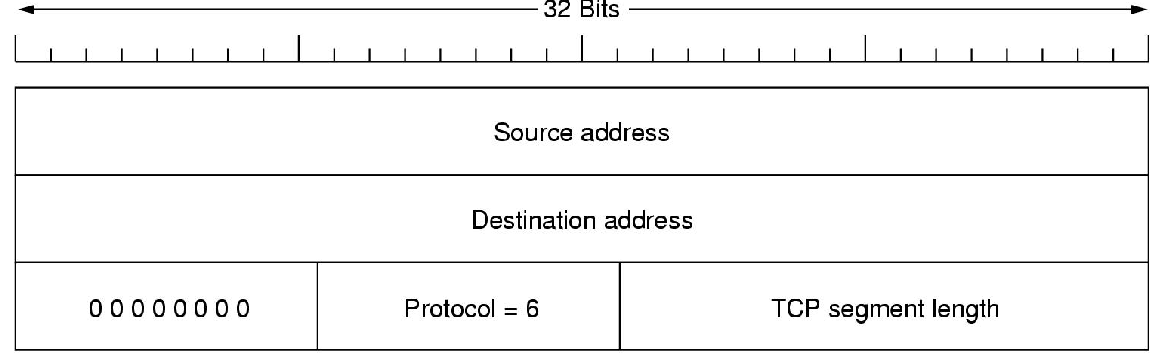
\includegraphics[width=0.42\textwidth]{pic/CN6/The pseudoheader of TCP}
        \caption{The pseudoheader of TCP}
    \end{figure}
    \item The Options field. may extended to 40 bytes to accommodate the longest TCP header 
    \begin{itemize}
        \item MSS(Maximum Segment Size), it defaults to a 536-byte load.
        \item The window scale negotiate a window scale factor at the start of a connection
        \item The timestamp 
        \item The SACK (Selective ACKnowledgement), is  used after a packet has been lost but subsequent (or duplicate) data has arrived. 
    \end{itemize}
\end{enumerate}

\subsubsection{TCP Connection Establishment}
Three Way Handshake
\begin{figure}[!htb]
    \centering
    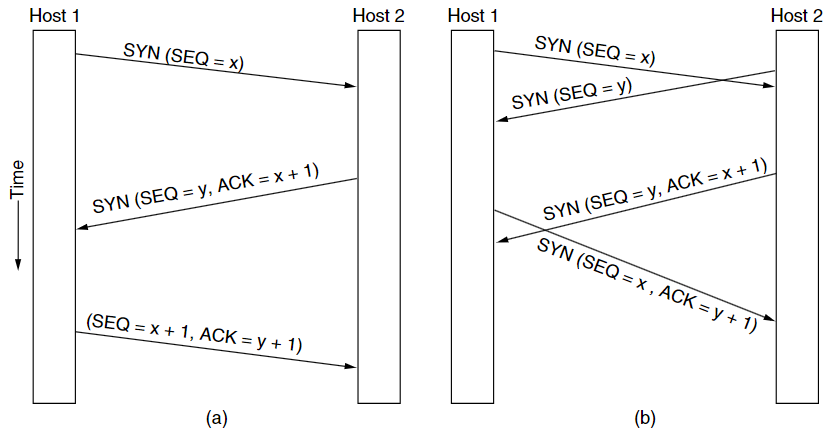
\includegraphics[width=0.42\textwidth]{pic/CN6/TCP Connection Establishment}
    \caption{(a) TCP connection establishment in the normal case. (b) Simultaneous connection establishment on both sides.}
\end{figure}

\begin{enumerate}
    \item Note that a SYN segment
    consumes 1 byte of sequence
    space so that it can be
    acknowledged unambiguously.
    \item The initial sequence number
    chosen by each host should
    cycle slowly. This rule is to
    protect against delayed
    duplicated packets.    
\end{enumerate}

\begin{enumerate}
    \item SYN --- for establishing a connection
    \subitem Request segment contains the following information in TCP header:
    \begin{enumerate}\scriptsize
        \item Initial sequence number (randomly chosen by the client)
        \item SYN bit set to 1.
        \item Maximum segment size
        \item Receiving window size (the limit of unacknowledged data that can be sent to the client, contained in the window size field)       
    \end{enumerate}
    \item SYN + ACK --- After receiving the request segment
    \subitem Reply segment contains the following information in TCP header:
    \begin{enumerate}\scriptsize
        \item Initial sequence number (randomly chosen by the server)
        \item SYN bit set to 1.
        \item Maximum segment size
        \item Receiving window size
        \item Acknowledgement number
        \item ACK bit set to 1. 
    \end{enumerate}
    \item ACK --- After receiving the reply segment
    \subitem sending a pure acknowledgement. Not necessary. 
\end{enumerate}

\paragraph{Important Points}\quad

\begin{itemize}\small
    \item Connection establishment phase consume 1 sequence number of both sides. But pure acknowledgement do not consume any sequence number. 
    \item Pure acknowledgement for the reply segment is not necessary. Client sending the data packet immediately can be considered as an ack. 
    \item For all the segments except the request segment, ACK bit is always set to 1.
    \item Certain parameters are negotiated during connection establishment. 
    \begin{enumerate}
        \item Window size
        \item Maximum segment size
        \item Timer values
    \end{enumerate}
    \item In any TCP segment
    \begin{itemize}\scriptsize
        \item If SYN bit = 1 and ACK bit = 0, then it must be the request
        segment.
        \item If SYN bit = 1 and ACK bit = 1, then it must be the reply segment.
        \item If SYN bit = 0 and ACK bit = 1, then it can be the pure ACK or segment meant for data transfer.
        \item If SYN bit = 0 and ACK bit = 0, then this combination is not possible.
    \end{itemize}
\end{itemize}